%-------------------------------------------------------------------------------
% yum_banks_and_roots
%-------------------------------------------------------------------------------
%
% \file        yum_banks_and_roots.tex
% \library     Documents
% \author      Chris Ahlstrom
% \date        2015-09-06
% \update      2016-03-01
% \version     $Revision$
% \license     $XPC_GPL_LICENSE$
%
%     Provides the concepts.
%
%-------------------------------------------------------------------------------

\section{Banks and Roots}
\label{sec:banks_and_roots}

   In recent versions of \textsl{Yoshimi}, the concepts of banks and roots
   have undergone a fair amount of change, including new features to make
   them easier to manage and easier to automate.  There are a lot of details
   to understand, too many to include along with the descriptions of the
   user-interface elements that control them.
   Therefore, this new section is devoted to banks and roots.
   It is an elaboration of material originally presented in
   \sectionref{subsec:concepts_banks_and_roots}.

   At one time, one could in theory have 1000 roots, 1000 banks and 1000
   presets.  However, now roots and banks were trimmed to what can be
   addressed from MIDI. One can supposedly still have 1000 presets, though.
   Anyway, 128x128x160 = 2621440 instruments should be enough for anyone.

   All root, bank, and instrument IDs are used by MIDI controls, and as of
   version 1.3.6 will also be accessible to the command line.

   The file \texttt{Banks.txt} in the \textsl{Yoshimi} source-code bundle
   makes an important point about a transition (in newer versions)
   to tagging roots (directories) and banks with an ID code:

   \begin{quotation}
      One no longer has the concept of a default root directory, but a current
      one. This can by changed at any time without requiring a restart, so
      there is no longer a need to display the (confusing) contents of all
      roots. Also, roots now have ID numbers associated with them, but no
      changes have been made to the actual directores to achieve this. Instead
      the IDs are stored in the config file. The same ID system is used for
      banks, again without making any file system changes.

      At first run (and whenever new root directories are set) unknown roots
      and banks are given these IDs. Once set they will not change no matter
      how many more roots and banks are later added. One can however, manually
      change root directory IDs in the 'Bank Root Paths window' accessible from
      the 'Paths' item in the main window. Also, there is a new Banks window so
      that these can be set up, moved and renamed in exactly the same way as
      instruments can.  With these IDs, roots and banks can be grouped/ordered
      by function instead of alphabetically. When using the GUI, one will
      always know exactly which root and bank one fetches an instrument from.

      One can quickly step between roots, banks and instruments with the so
      marked buttons in each of these, and if one right-clicks on them one will
      close one window as one opens the other.

      The significance of all this is that one's MIDI sequencer can now
      reliably use these ID numbers to select roots, banks and (already
      available) instruments. That Rosegarden or Muse file one saves today will
      be just as valid in the future, unless one makes the deliberate choice to
      change some IDs. Indeed, one can now start with an 'empty'
      \textsl{Yoshimi}, and
      via MIDI, set roots, banks and load instruments into parts (enabling the
      parts as one does so) swapping banks and roots as necessary. While the
      MIDI file runs it can silently pull instruments from any root/bank into
      any non-sounding part without disturbing the playing ones.

      In Yoshimi / Settings / MIDI one can enable or disable all these features,
      and can define which CCs one wants to use. Bank can be Off, MSB or LSB
      (as before). Since V1.5.11 Root can also be Off, MSB or LSB.
      Also, Extended Program Change now has the restriction of not being any
      reserved CC. These three are all cross-checked against each other.
      As an example, one might set Bank to LSB amd Root to MSB, effectively
      giving one extended bank control compatible with all sequencers.

      Also, different instances have their own config files so that one can
      have (say) the main instance with current root(9), bank(23) while
      instance 4 has current root(2), bank(6). One can call up instances by
      number and thus access saved settings for that instance. As each instance
      has its own MIDI and audio ports, they can behave more-or-less
      independently.

      In doing all of this we have completely changed the way we manage the
      structure internally, resulting in much greater efficiency, at the cost
      of only a slightly slower startup. Swapping roots performs *no* file
      operations. Swapping banks only fetches the directory list of the newly
      selected bank. Changing an instrument doesn't have to search for a file,
      only load from its already known location.

      If one changes a bank root path, either through the gui or via MIDI, it
      will always reset the current bank to the lowest numbered one it can
      find. This is because there may not be a bank in the new root with the
      same ID, and even if there is, there is no guarantee that it will have
      the same name or contents.

      Also if an attempt is made to reload the same root, nothing will actually
      happen. The same is true of banks. Both of these are kept fully
      up-to-date so there would be no point.

      However, reloading the same *instrument* will be performed every time, as
      one may have changed what is currently loaded without saving it. This
      provides an effective 'restore' operation.

      Finally, it is generally advisable to make root and bank changes on
      channel 1 so that one can more easily keep track of them. However they
      are not channel sensitive as they don't directly affect the sound, so one
      can set them in any convenient channel then perform individual program
      changes on the desired channels.
   \end{quotation}

   It has always been possible to swap and move instruments within a bank, and
   since V 1.3.5 it was possible to swap banks within a bank root, but now one can
   swap/move instruments across any banks and any bank roots. One can also move
   whole banks across bank roots.  These extensions use exactly the same controls
   as before. However, it isn't just a case of changing IDs. Files are actually
   moved, so additional protections and warnings are put in place.

   There are also bank importing and exporting controls and since version 1.5.8
   these have been made available to the CLI with specific IMport and EXPort
   controls.

   A "CC" is a MIDI "continuous controller".
   A MIDI bank change is usually a CC\#0 value of 0, followed by a CC\#32
   value of X, where X is the desired bank number from 0 to whatever.
   (However, in some cases it may simply be a CC\#0 on its own with a value
    of X).  Many synths also require that one send a program change after
   the bank change, to select the program within the bank.

\subsection{Roots}
\label{subsec:banks_and_roots_roots}

   In \textsl{Yoshimi}, a \textsl{root} is a location in which banks can be
   stored.  It is basically a directory, though it ultimately is assigned a
   number by \textsl{Yoshimi}, so that it can be accessed in an automated
   way.  By choosing a root and making it the current root, one can hone in
   on a smaller collection of banks.

   One cannot reach root paths through the \textbf{Yoshimi / Settings} menu
   any more; it was causing a nightmare of syncing with the other entry
   routes. One can reach it from the Banks window
%  (see \sectionref{subsubsec:menu_instrument_show_banks})
   or the Instruments window,
%  (see\sectionref{subsubsec:menu_instrument_show}),
   and both of the latter also have multiple entry routes.
   Roots can also be reached through the \textbf{Yoshimi / Paths} menu.

\subsection{Banks}
\label{subsec:banks_and_roots_banks}

   Another important concept in \textsl{Yoshimi} is \textsl{banks}.  Instruments
   can be stored in banks. These are loaded and saved automatically by the
   program.  On program start, the last used bank is loaded. A single bank
   can store up to 128 instruments normally, and 160 using extended programs.

%  TODO:  We should be able to walk the user through a session and
%  set up a set of instruments that is tractable under MIDI control.
%  \index{todo!banks/roots}

%  MOVED SOMEWHERE ELSE IN Menu:
%
%  Some minor instructions are provided in
%  \sectionref{subsubsec:menu_instrument_show_root_paths}.

   Also note that, as well as bank and program changes, there is the ability
   to set a MIDI CC to access the voices from 129 to 160 (numbered re 1).
   All the Bank controls are contained in a tab in the main
   \textbf{Settings} window, and take immediate effect.

   Bank root directories are identified with ID numbers that can be changed
   by the user in the user-interface. This feature is also made available for
   selection over MIDI.  MIDI only sees banks in the \textsl{current} root
   directory, but all banks are accessible to the user-interface.

\subsubsection{Bank Directories}
\label{subsubsec:banks_and_roots_bank_directories}

   Banks are arranged in directories, with each directory containing a number
   of instrument files.

   Each instrument's file-name should begin with a 4-digit number
   (left-padded with 0's to make it 4 digits long).  This number can serve
   as a MIDI patch number for automated selection of the instrument via a
   MIDI program-change message.

   Unnumbered instruments in a bank will be given a temporary ID starting
   from number 160 and working down. If those numbers already exist then
   they will be skipped over. This can get very confusing. However, if one
   simply loads it and re-saves it to the same instrument slot, it will gain
   that ID and be properly fixed.  One can then move-swap it with others.

   See also \sectionref{subsubsec:menu_patch_sets}, and
   \sectionref{sec:banks_collection}, for further information.

   In \textsl{Yoshimi} V 1.7.1 there has been further restructuring of banks to
   make them not only more efficient, but also provide additional protections and
   capability.

   The first of these copies all banks found in the non-editable locations /usr
   and /usr/local into the users hidden directory .local/share. It only does this
   if they are not already there, and for first time users silently adds these to
   priority locations in the recognised bank roots. One now has fully editabe
   banks and roots, but still has the protection of non-writable ones.

   For existing users, the copying process takes place, but the banks are not
   automatically installed. Instead one is presented with the following dialog.

\begin{figure}[H]
   \centering
   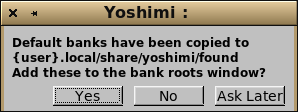
\includegraphics[scale=0.75]{1.7.1/Banks_Checked.png}
   \caption{Bank Install Dialog}
   \label{fig:bank_install_dialog}
\end{figure}

   With either 'Yes' or 'No' one will not be asked again, so if in doubt it is
   advisable to select 'Ask Later'

   Another upgrade resolves a problem where it is possible to start with no banks
   at all. Ths could be due to an accidental deletion, or, for a new user, an
   installer may not have included them. In this situation Yoshimi will generate
   a new bank root, bank and instrument and make these available.

   A similar problem is where one tries to add a new bank root that doesn't
   actually exist. Previously \textsl{Yoshimi} would just report this and close
   the operation. Now you will see the following dialog.

\begin{figure}[H]
   \centering
   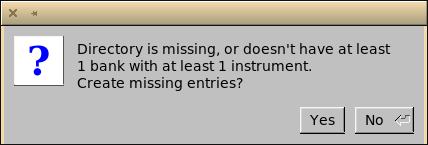
\includegraphics[scale=0.75]{1.7.1/No_Root.png}
   \caption{Root Not Found Dialog}
   \label{fig:no_root_dialog}
\end{figure}

If one selects 'Yes' \textsl{Yoshimi} will create and install the bank root asked for and will create 'newBank' in it, and inside that '0005-First Instrument' which will be a quite nice SubSynth one. It will also load that instrument to part 1.

The last improvement provided by \textsl{Yoshimi} V 1.7.1 concerns banks having additional entries installed by external means, such as from the OS filing system. This is always advised against, partly because one doesn't necessarily know exactly what is there, but also because, previously, it would cause Yoshimi to regenerate the entire bank root which would result in different IDs for existing ones, thus breaking one's older projects.

The new behaviour is to first install banks Yoshimi already knows about, and then test validity and install any new ones in spaces between the others. We still advise against doing this. It is much better to use the Install routine provided in the Banks window.

%-------------------------------------------------------------------------------
% vim: ts=3 sw=3 et ft=tex
%-------------------------------------------------------------------------------
